\appendix
% remove header trickery
\chapter[]{Anhang}
\addcontentsline{toc}{chapter}{A\ \ Anhang}
\begin{table}[H]
    \caption{Spannungswerte bei der Konditionierung}
    \label{tab:Konditionierung}
    \begin{tabular}{lccc}
        \toprule
        Spannungsdifferenz [V] & Strom [mA] &	Widerstand [M$\Omega$] & Zeitinterval [min]\\   
        \midrule
            880  & 0,018 & 48,9 & 05:57\\
            980  & 0,021 & 46,7 & 06:39\\
            1080 & 0,024 & 45,0 & 05:36\\
            1200 & 0,028 & 42,9 & 07:26\\
            1330 & 0,032 & 41,6 & 07:20\\
            1450 & 0,036 & 40,3 & 04:13\\
            1580 & 0,040 & 39,5 & 04:41\\
            1700 & 0,044 & 38,6 & 04:43\\
            1825 & 0,048 & 38,0 & 06:01\\
            1940 & 0,052 & 37,3 & 05:10\\
            2060 & 0,056 & 36,8 & 07:45\\
            2160 & 0,059 & 36,6 & 05:57\\
            2270 & 0,063 & 36,0 & 05:59\\
            2380 & 0,068 & 35,0 & 06:16\\
            2480 & 0,071 & 34,9 & 06:27\\
            2600 & 0,071 & 36,6 & 06:02\\
            2700 & 0,080 & 33,8 & 06:46\\   
        \bottomrule     
    \end{tabular}
\end{table}


\begin{figure}[H]
    \centering
    \hspace{-1.5cm}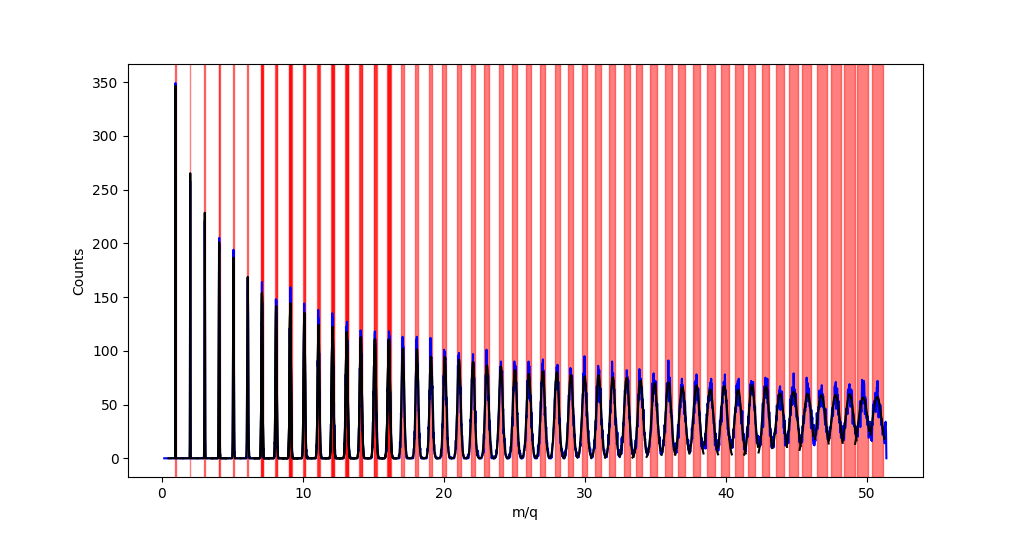
\includegraphics[width=1.1\textwidth]{Resolution_intergration.png}
    \caption[Gauß-Fit und Integrationsgrenzen bei Bestimmung der Auflösung]{Gauß-Fit und Integrationsgrenzen bei Bestimmung der Auflösung bei einer Detektordistanz von 410 mm. Der Fit ist in Schwarz dargestellt, die Integrationsgrenzen in Rot und die leicht gefilterten Daten in Blau.}
    \label{fig:integrationsgrenzen}
\end{figure}
\clearpage
\section{Ergänzendes zur Simulation}
Alle Skripte sowie die gesamte ionenoptische Simulation, die im Verlauf dieser Arbeit entwickelt wurden, stehen zur freien Verfügung und sind im GitLab der JLU Gießen unter folgendem Link zu finden: \url{https://gitlab.ub.uni-giessen.de/so9354/zerob-software}.



\begin{figure}[H]
    \centering
    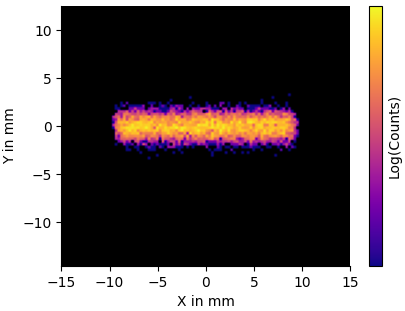
\includegraphics[width=.55\textwidth]{Pos_210.png}
    \caption[Positionsplot des konvergenten Strahls]{Positionsplot des konvergenten Strahls bei einer Flugstrecke von 210 mm.}
    \label{fig:pos_210}
\end{figure}

\begin{figure}[H]
    \centering
    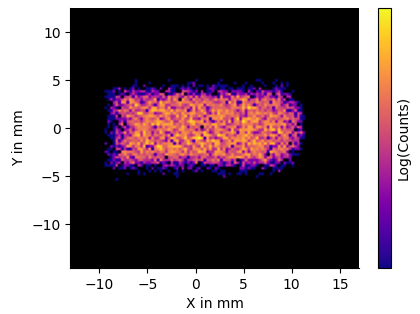
\includegraphics[width=.55\textwidth]{Pos_Forward_Bias.png}
    \caption[Positionsplot mit Vorzugsrichtung der thermischen Bewegung]{Positionsplot mit Vorzugsrichtung der thermischen Bewegung der Ionen. Die Richtungsverteilung der thermischen Bewegung (hier 1/5 eV) ist in einem Kegel um die x-Achse gegeben. Der Öffnungswinkel des Kegels beträgt 110°. Versucht wurde die Verschiebung in x-Richtung des Strahl im Expermiments nachzuvollziehen. Allerdings ist kein wesentlicher Unterschied zu Abbildung \ref{fig:sim_pos_kinetic} erkennbar.}
    \label{fig:pos_bias}
\end{figure}   


\begin{figure}[H]
    \centering
    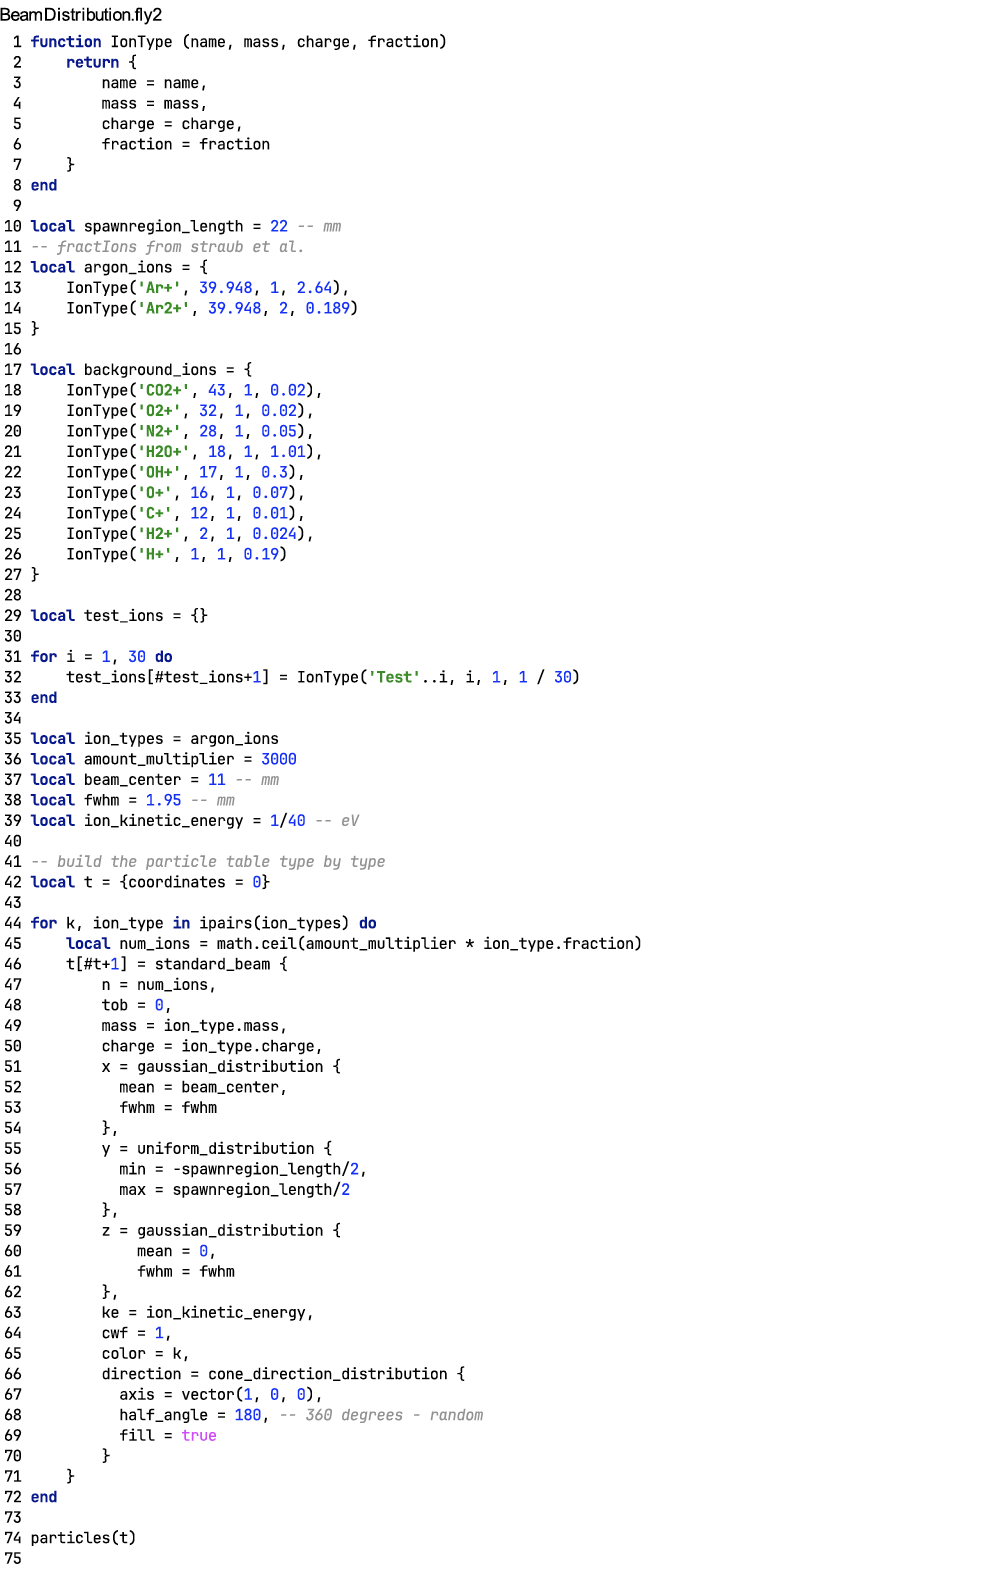
\includegraphics[width=1.05\textwidth]{Fly2.png}
    \caption[Ionenverteilung .fly2-File]{\textsc{.fly2}-File zur Definition der Ionenverteilung in \textit{SIMION} in der Programmiersprache Lua.}
    \label{fly2}
\end{figure}